\documentclass[english,11pt]{beamer}

\setlength{\parskip}{\smallskipamount}
\setlength{\parindent}{0pt}

\setbeamersize{text margin left=10pt, text margin right=10pt}

\renewcommand{\imath}{\mathfrak{i}}
\newcommand{\emath}{\mathrm{e}}

\usepackage{minted}
\newminted{text}{breaklines,fontsize=\footnotesize}
\newminted{bash}{breaklines,fontsize=\footnotesize}

\begin{document}

\title{Introduction to Linux Command Line Interface}
\author{Fadjar Fathurrahman}
\institute{Department of Engineering Physics\\
Research Center for Nanoscience and Nanotechnology\\
Bandung Institut of Technology}
\date{}
\maketitle

\begin{frame}
\frametitle{Overview}

This talk is intended to teach the basics of working with
command line interface (CLI) of Linux for those who never
used CLI before.

From Wikipedia:

\begin{quotation}
A command-line interface (CLI) is a means of interacting with a computer
program where the user (or client) issues commands to the program in the
form of successive lines of text (command lines).
The interface is usually implemented with a command line \textbf{shell}
\end{quotation}

We will limit our discussion to \textbf{bash} shell because this is the most popular
shell in Linux.
\end{frame}


\begin{frame}
\frametitle{Command line interface}

Advantages:
\begin{itemize}
\item Requires fewer resources
\item Concise and powerful
\item Expert-friendly
\item Easier to automate via scripting
\end{itemize}

Disadvantages
\begin{itemize}
\item Unintuitive
\item Commands not obvious
\item Not visually rich
\item Beginner-unfriendly
\end{itemize}

\end{frame}


\begin{frame}
\frametitle{Accessing command line interface}

There are at least two ways of doing this:
\begin{itemize}
\item Via menu: \textsf{Accessories} →  \textsf{Terminal}
\item Using special shortcut: \textbf{Ctrl + Alt + T} (on Ubuntu)
\end{itemize}

{\centering
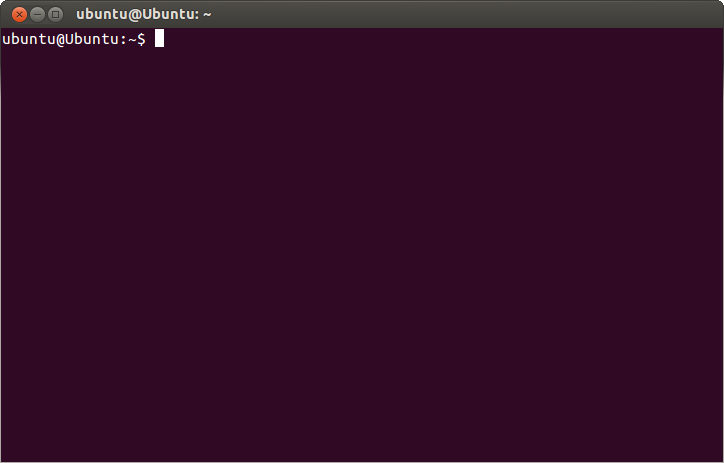
\includegraphics[scale=0.25]{images/terminal_ubuntu.png}
\par}

\end{frame}



\begin{frame}[fragile]
\frametitle{Displaying text on screen}

Type the following (and press enter at the end of line)
\begin{bashcode}
echo "My name is XXX"
echo My name is XXX
\end{bashcode}

Both will result in the same output.

I personally prefer the first style.
\end{frame}


\begin{frame}[fragile]
\frametitle{Working with variables}

Built-in variable \texttt{USER}
\begin{bashcode}
echo $USER
# to access the variable we append a dollar sign in front
# of the variable name

echo USER  # notice that there is no dollar sign

echo "Hello, I am logged in as $USER"
\end{bashcode}

Define new variable: (Note that there is no space after variable name)
\begin{bashcode}
MYNAME="Fadjar Fathurrahman"
echo "Hello, my name is $MYNAME"
\end{bashcode}
%stopzone

Be careful with space(s)
\begin{bashcode}
MYNAME=Fadjar Fathurrahman # will result in error
\end{bashcode}

\end{frame}


\begin{frame}[fragile]
\frametitle{Working with variables (cont'd)}

Define a variable named \verb|AWESOME_ACTORS|:
\begin{bashcode}
AWESOME_ACTORS="Johnny Depp, Morgan Freeman"
echo $AWESOME_ACTORS
\end{bashcode}
%stopzone

Add some actors to \verb|AWESOME_ACTORS|:
\begin{bashcode}
AWESOME_ACTORS="Samuel L Jackson, Robert Downey Jr., $AWESOME_ACTORS"
echo $AWESOME_ACTORS
\end{bashcode}

Redefine \verb|AWESOME_ACTORS|
\begin{bashcode}
AWESOME_ACTORS="Christian Bale, Matt Damon"
echo $AWESOME_ACTORS
\end{bashcode}
%stopzone

\end{frame}


\begin{frame}[fragile]
\frametitle{Working with variables (cont'd)}

Other useful built-in variables:
\begin{bashcode}
echo $PATH
echo $LD_LIBRARY_PATH
echo $HOME
\end{bashcode}
%stopzone

\verb|PATH| tells the shell which directories to search for executable files (i.e. ready
to run programs) in response to commands issued by a user.

\verb|LD_LIBRARY_PATH|
is similar to \verb|PATH|, but applies for libraries.

\verb|HOME|%stopzone
is location of user's home directory, usually \verb|/home/username|.
It can be shortened using \verb|~|.

\end{frame}


\begin{frame}[fragile]
\frametitle{Files and directories}

\begin{bashcode}
pwd # display current directory
ls  # display list of files in current directory
\end{bashcode}

Go to specific directory (changing directory)

\begin{bashcode}
cd SecretDirectory  # go to a directory with name SecretDirectory
cd ../              # go "up"
cd $HOME            # go to home directory
cd                  # same as cd $HOME
cd /                # go to directory /
\end{bashcode}

Create new directory
\begin{bashcode}
mkdir MyNewSecretDirectory
\end{bashcode}

\end{frame}


\begin{frame}[fragile]
\frametitle{Files and directories (cont'd)}

Be careful with spaces: (again)
\begin{bashcode}
mkdir My New Secret Directory # will create several directories
mkdir "My New Secret Directory"
cd My New Secret Directory   # will go to the first directory, i.e. My
cd "My New Secret Directory"
\end{bashcode}

To delete files we can use the command \verb|rm|. To delete a directory we can use
\verb|rm -r|
\begin{bashcode}
rm MySecretFile.txt      # delete a file
rm -r MySecretDirectory  # delete a directory (and all files in it)
\end{bashcode}

\verb|rm| command is considered VERY DANGEROUS. Be careful when using it.

\end{frame}



\begin{frame}[fragile]
\frametitle{Files and directories (cont'd)}

To \textbf{rename} a directory or a file we can use the command \verb|mv|
\begin{bashcode}
mv DirName BetterDirName
mv OldName.txt NewName.txt
\end{bashcode}

Command \verb|mv| also can be used to \textbf{move files and directories} to
another directory:
\begin{bashcode}
mv file1.txt file1.txt dir2 dir2 DestinationDir
\end{bashcode}

\end{frame}


\begin{frame}[fragile]
\frametitle{Files and directories (cont'd)}

The \verb|cp| command can be used to \textbf{copy} files.

Copy \verb|file1| to \verb|file2|
\begin{bashcode}
cp file1 file2
\end{bashcode}

Copy two files from upper directory to current directory ('./' or simply '.')
\begin{bashcode}
cp ../file1 ../file2 ./
\end{bashcode}

Copy directory \verb|dirname| to current directory
\begin{bashcode}
cp -r ~/dirname/ ./
\end{bashcode}

\end{frame}


\begin{frame}[fragile]
\frametitle{Files and directories (cont'd)}

The command \verb|ls| has several options:
\begin{bashcode}
ls
ls -l
ls -al
ls -alh
\end{bashcode}

List all files in a directory named \verb|MySecretDirectory|:
\begin{bashcode}
ls MySecretDirectory
ls -l MySecretDirectory
ls -al MySecretDirectory
ls -alh MySecretDirectory
\end{bashcode}

\end{frame}


\begin{frame}[fragile]
\frametitle{Text editor(s)}

Create empty file:
\begin{bashcode}
touch A_Whole_New_File.txt
\end{bashcode}

Edit the file (use either nano or gedit)
\begin{bashcode}
nano A_Whole_New_File.txt
gedit A_Whole_New_File.txt &
\end{bashcode}

Type the following (or other text if you wish)
\begin{bashcode}
A whole new file
A new fantastic point of view
No one to tell us no
Or where to go
Or say we're only dreaming
\end{bashcode}

\end{frame}


\begin{frame}[fragile]
\frametitle{Text editors (cont'd)}

{\centering
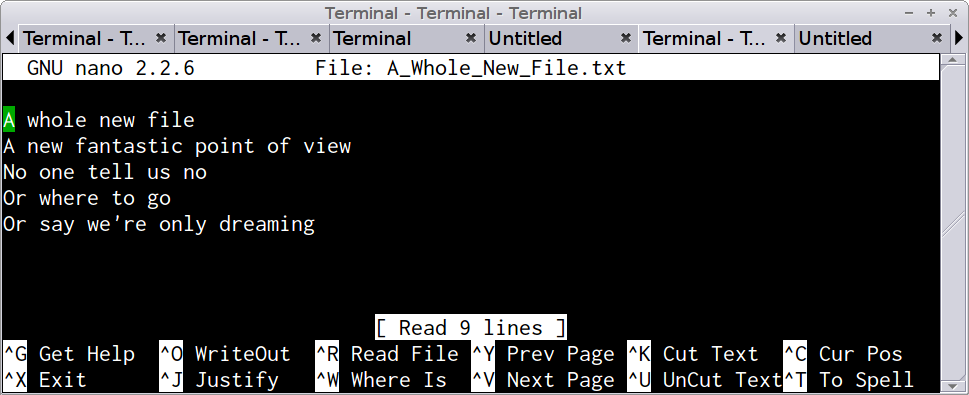
\includegraphics[scale=0.25]{images/nano1.png}
\par}

\verb|nano| is more difficult to use as compared to \verb|gedit|.

\verb|gedit| is very much like Notepad in Windows.

\end{frame}


\begin{frame}[fragile]
\frametitle{Text editors (cont'd)}

\verb|less| can be used if we only interested in viewing the content
of a text file. For example try:
\begin{bashcode}
less A_Whole_New_File.txt
\end{bashcode}

To quit from \verb|less| type \verb|q|.

There are a lot of text editors on Linux:
\begin{itemize}
\item vim (\url{http://www.vim.org})
\item emacs (\url{www.gnu.org/software/emacs})
\item Visual Studio Code (\url{https://code.visualstudio.com/})
\item See the list on Wikipedia \url{https://en.wikipedia.org/wiki/Category:Linux_text_editors}
\end{itemize}

Interesting read: \url{https://en.wikipedia.org/wiki/Editor_war}

\end{frame}



\begin{frame}[fragile]
\frametitle{Redirection and pipelining}

Sometimes, we want to save what displayed after in the terminal after
calling a command/program. We can do this by \textit{redirecting} the output
to another file (usually a text file).
\begin{bashcode}
ls -lh > file_list.txt
less file_list.txt
\end{bashcode}

If we want the output to be displayed in the terminal and also written
in a file, we can use \verb|tee|.
\begin{bashcode}
ls -lh | tee file_list.txt
\end{bashcode}
Note that in the previous example, we also have used \textbf{pipelining} by
using the character \texttt{|}. This will take the output of the first command,
i.e. \verb|ls -lh| and supplied it to \verb|tee| which will display and write
to a file.

\end{frame}



\begin{frame}[fragile]
\frametitle{Input and output file}

In the following workshops, we will work with various programs.

These programs usually need to read an input file.

The input file can be provided by redirection using symbol \verb|<| (in this
case, the program read the input file from standard input)
\begin{bashcode}
AProgram < input_file
\end{bashcode}

Other programs may need to be supplied input file name as an argument to
the program
\begin{bashcode}
AnotherProgram input_file
\end{bashcode}
\end{frame}


\begin{frame}[fragile]
\frametitle{Input and output file (cont'd)}

In most cases, the program will give some messages or important output on
the standard output (screen).

If this is the case, the we may use the following to redirect the output
to a file:
\begin{bashcode}
AProgram < input_file > log_file
AnotherProgram input_file > another_log_file
\end{bashcode}

\end{frame}


\end{document}
